\chapter{Homework 9}

\section{Problem 1}

\newcommand{\ns}{\not \sim}

\begin{tabular}{|c|c|c|c|c|} \hline
    -               & $\text{TS}_1$ & $\text{TS}_2$ & $\text{TS}_3$ & $\text{TS}_4$ \\ \hline
    $\text{TS}_1$   & -             & $\ns$         & $\ns$         & $\ns$         \\ \hline
    $\text{TS}_2$   & -             & -             & $\ns$         & $\ns$         \\ \hline
    $\text{TS}_3$   & -             & -             & -             & $\ns$         \\ \hline
    $\text{TS}_4$   & -             & -             & -             & -             \\ \hline
\end{tabular}

Reason for $\text{TS}_1 \ns \text{TS}_2$:

Consider the $t_3$ in $\text{TS}_2$. $\text{L}_2(t_3) = \{a, b\}$ and we have $t_3 \to t_1$, where $\text{L}_2(t_1) = \{a\}$.
If bisimulation holds, then there exists $x, y$ in $\text{TS}_1$, where we have:
$\text{L}_1(x) = \{a, b\}$, $x \to y$, and $\text{L}_1(y) = \{a\}$.

But we can't, so $\text{TS}_1 \ns \text{TS}_2$.

\section{Problem 2}

\subsection*{(a)}

The $\to$ direction is trivial, which can be simply solved by induction.
We will focus on the $\leftarrow$ direction.

Let $M = |S| \times |S| + 2$, we claim that if $s_1 \sim_{M} s_2$ holds, then
$\forall s_1' \in \text{Post}(s_1), \exists s_2' \in \text{Post}(s_2)$ such that $s_1' \sim_{M} s_2'$.
The reverse direction is similar.

First, we define $\text{Post}^{n}(s)=\{s'' | s' \in \text{Post}^{n-1}(s) \wedge s' \to s'' \}$, and
specially, $\text{Post}^{0}(s)=\{s\}$ (which means $\text{Post}^{1}(s)=\text{Post}(s)$, following the
natural definition of $\text{Post}$).

Second, we introduce a lemma that for any $x$ if $s_1 \sim_{x + 1} s_2$ holds, then
$s_1 \sim_{x} s_2$ holds as well, which can be simply proved by induction (so we skip the proof).
This can extend to the fact that for any $x > y$, if $s_1 \sim_{x} s_2$ holds, then $s_1 \sim_{y} s_2$ holds as well.

Suppose our claim doesn't hold. By definition of $\sim_{M}$, for some $s_1' \in \text{Post}(s_1)$, there
exists $s_2' \in \text{Post}(s_2)$ such that $s_1' \sim_{M -1} s_2'$.
Since our claim doesn't hold, we have $s_1' \sim_{M-1} s_2'$ but $s_1' \ns_{M} s_2'$.

Similarly, for some $s_1'' \in \text{Post}(s_1')$, there exists $s_2'' \in \text{Post}(s_2')$ such that
$s_1'' \sim_{M-2} s_2''$ but $s_1'' \ns_{M-1} s_2''$.

Similarly, we derive such a sequence of $s_{1,n}, s_{2,n}$,
where $s_{1,n} \in \text{Post}^{n}(s_1)$, $s_{2,n} \in \text{Post}^{n}(s_2)$,
$s_{1,n} \sim_{M-n} s_{2,n}$ but $s_{1,n} \ns_{M-(n-1)} s_{2,n}$, and $1 \leq n < M$.

Since there's at most $|S| \times |S|$ state pairs, there must exist $1 \leq i < j \leq |S| \times |S| + 1 < M$,
such that $(s_{1,i}, s_{2,i}) = (s_{1,j}, s_{2,j})$. We denote this pair as $(x, y)$.

Then, we have $x \sim_{M - i} y$ but $x \ns_{M - i + 1} y$, and $x \sim_{M - j} y$ but $x \ns_{M - j + 1} y$.
However, since $i < j$, we have $M - j + 1 \le M - i$. When $j = i + 1$, $x \sim_{M - i} y$ conflicts with
$x \ns_{M - j + 1} y$. When $j > i + 1$, $x \sim_{M - i} y$ implies $x \sim_{M - j + 1} y$ by the lemma we introduced above,
which also indicates a contradiction.

As a result, we have proved that if $s_1 \sim_{M} s_2$ holds, then
$\forall s_1' \in \text{Post}(s_1), \exists s_2' \in \text{Post}(s_2)$ such that $s_1' \sim_{M} s_2'$.
For the reverse direction, we can prove similarly.

By definition, $\sim_{M}$ is a bisimulation relation, which implies $s_1 \sim_{TS} s_2$ holds.

\subsection*{(b)}

counterexample is:

\begin{figure}[H]
    \centering
    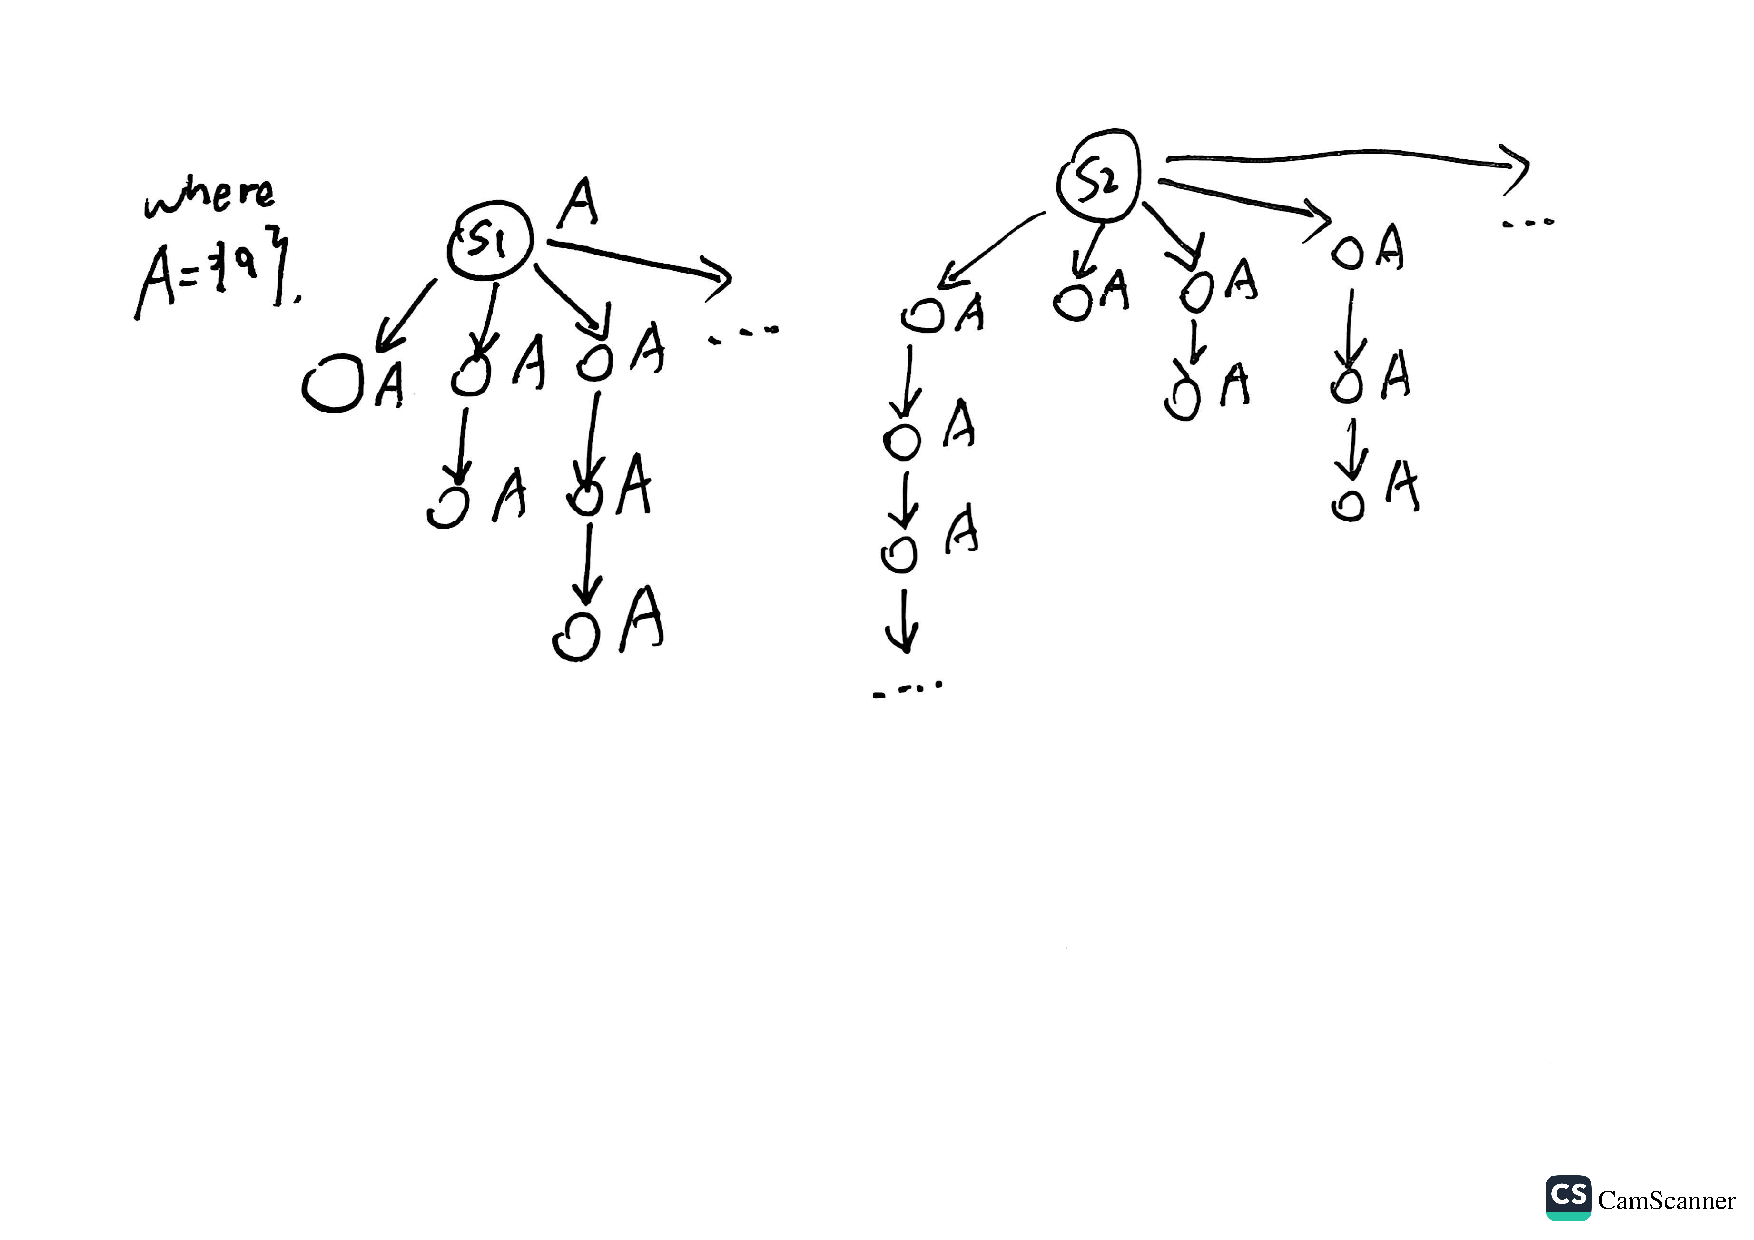
\includegraphics[width=0.8\textwidth]{hw9-counterexample.pdf}
    \caption{Counterexample for Problem 2(b)}
\end{figure}

Note that there's a missing label $A$ for $s_2$ in the image.

Trivially, for any given $n$, we have $s_1 \sim_{n} s_2$ holds. The state that can accept infinitely many $\{a\}$
in $\text{Post}(s_2)$ has $\sim_{n}$ relation with the state in $\text{Post}(s_1)$ that can accept at least $n + 1$ $\{a\}$.

However, there doesn't exist a state in $\text{Post}(s_1)$ that can accept infinitely many $\{a\}$,
so we don't have $s_1 \sim_{TS} s_2$ holds.

In fact, I think this is the difference between arbitrary any finite $n$ and the infinite.
